% Generated from main.typ. Typst is authoritative; regeneration overwrites this file.
\documentclass{qlnotes-export}

\title{MATH 597: Measure Theory}
\subtitle{Typst-first course notes and worked homeworks}
\author{Qiulin Fan}
\date{Winter 2025}

\begin{document}
\mainmatter
\chapter{Hardy-Littlewood maximal function and Lebesgue differentiation theorem}\label{hardy-littlewood-maximal-function-and-lebesgue-differentiation-theorem}

\section{Hardy-Littlewood max function and max theorem {[}Fol 3.4{]}}

目前我们 finish 了 Folland 的 Ch1, Ch2.\\
我们将先跳过 Radon-Nikodym differentiation theory, 在讲完 \(L^{p}\) space theory 后再回到 Radon-Nikodym differentiation theory. 但是我们将会先将 differentiation theory 中的一个特殊部分: HL max theorem 和 Lebesgue differentiation theorem, 因为它们在 \(L^{p}\) space theory 中需要被用到.\\
此 lec 对应: Folland 3.4( 1)\\
Differentiation theorey 的 overview:\\
Radon-Nikodym derivative 并不是 classical calculus 的扩展 (classical calculus 表示变量之间的相对变化), 而是专门针对: 同一个 measure space 上, 一个测度对于另一个测度 (要求它们之间绝对连续) 的变化率.

\[d\nu = fd\mu\]

从而

\[\nu(A) = \int_{A}f d\mu\]

这使得我们可以更改一个积分 with respect to 的测度.\\
\strut \\
其核心定理: Radon-Nikodym Theorem, 表示了在一般的 measure space 上, 这两个测度满足一定条件下, 这个 Radon-Nikodym derivative 的存在性; 而 LDT 提出一种\textbf{在 Euclidean space 上, 求 Radon Dikodym derivative 的方法.}\\
LDT 本身是一种将积分信息转换为点态信息的手段. 它表示\textbf{对于 locally integrable 的函数, 局部积分平均值可以收敛到函数本身, a.e.}\\
因而在知道 \(\nu\) 和 \(\mu\) 的情况下, LDT 提供了类比经典微积分中 "导数是局部变化率的极限" 的观点: 在 Euclidean space 上, Radon Nikodym derivative 等于局部均值:

\[f(x) = \lim\limits_{r\rightarrow 0}\frac{\nu(B(r,x))}{\mu(B(r,x))}\text{for a.e.}\ x\]

Radon Nikodym derivative 的应用: 比如在概率论中, \textbf{pdf/pmf 都是 cdf 对于 Lebesgue measure 的 Radon Nikodym derivative}; 在贝叶斯推理中，给定先验 prior 和观测数据的分布, 后验分布 posterior 的密度可以通过 Radon-Nikodym 导数计算. 下面介绍概念:\\
\strut \\

\subsection{\texorpdfstring{\(L_{loc}^{1}\) and local average}{L\_\{loc\}\^{}\{1\} and local average}}\label{l_loc1-and-local-average}

\begin{definition}{\protect\phantomsection\label{kn-locally-integrable}{\textbf{locally
integrable}}}

如果 measurable \(f:{\mathbb{R}}^{n}\rightarrow{\mathbb{C}}\) 在任意 bounded subset of \({\mathbb{R}}^{n}\) 上的 integral 都 \(< \infty\), 则称 function \(f:{\mathbb{R}}^{n}\rightarrow{\mathbb{C}}\) 是 locally integrable 的, 写作 \(f \in L_{loc}^{1}(m)\).

\end{definition}

\begin{qlremark}{Remark}

等价于 \(f\) \textbf{在任意 compact set 上}的 integral 都 \(< \infty\):

\[\int_{K}f dm < \infty\]

for all \(K\) ; 或者\(f\) \textbf{在任意 open ball 上}的 integral 都 \(< \infty\):

\[\int_{B(r,x)}f dm < \infty\]

for all \(x,r\).\\
这是比 \(f \in L^{1}(m)\) 更弱的条件. For example: 连续函数一定是 \(L_{loc}^{1}\) 的.

\end{qlremark}

\begin{example}

考虑

\[\left. f(x) := \middle| x \middle| {}_{p},\quad x \in {\mathbb{R}}^{n} \right.\]

(使用 polar coord) 可验证:

\[f \in L_{loc}^{1}(m)\quad\Leftrightarrow\quad p > - n\]

\end{example}

\begin{definition}{\protect\phantomsection\label{kn-average}{\textbf{average}}}

对于 \(f \in L_{loc}^{1}(m)\), 以及 bounded and Lebesgue measurable \(E \subset {\mathbb{R}}^{n}\) with \(m(E) > 0\), 我们定义:

\[\text{avg}_{E}f: = \frac{1}{m(E)}\int_{E}f dm\]

为 \(f\) 在 \(E\) 上的 \textbf{average value}.\\
特别地, 当 \(E\) 为一个 ball \(B(r,x)\) 时, 我们可以写作:

\[A_{r}f(x) := \text{avg}_{B(r,x)}f\]

表示它在 \(x\) 为中心的 \(r\) 为半径的 ball 上的 average.

\end{definition}

\begin{lemma}

对于任意 \(f \in L_{loc}^{1}\), \(A_{r}f(x)\) 都是 jointly continuous in \(r\) and \(x\) 的. (\(r > 0,x \in {\mathbb{R}}^{n}\))

\end{lemma}

\begin{proof}

Suppose \((x_{j},r_{j})\rightarrow(x,r)\) in \({\mathbb{R}}^{n} \times {\mathbb{R}}_{> 0}\).\\
于是 for sure:

\[m(B(x_{j},r_{j}))\overset{j\rightarrow\infty}{\rightarrow}m(B(x,r))\]

并且 by DCT (取 \(\chi_{B(r_{0} + 1,x_{0})}\) 作为 bound) 可以得到:

\[\int f\chi_{B(x_{j},r_{j})}\rightarrow\int\chi_{B(x,r)}\]

\end{proof}

\subsection{Hardy-Littlewood maximal function}\label{hardy-littlewood-maximal-function}

\begin{definition}{\protect\phantomsection\label{kn-hardy-littlewood-maximal-function}{\textbf{Hardy-Littlewood
maximal function}}}

对于 \(f \in L_{loc}^{1}\), 我们定义它的 HL maximal function 为:

\[\left. Hf(x): = \sup\limits_{r > 0}A_{r} \middle| f \middle| (x) \right.\]

\end{definition}

HF maximal 函数 \(Hf(x)\)表示 \(f\) 的绝对值函数在 \(x\) 处能取到最大的 local average.

\begin{theorem}{\protect\phantomsection\label{kn-hl-maximal-function-measurable}{\textbf{HL
maximal function 是 measurable 的}}}

对于任意 \(f \in L_{loc}^{1}\), \(Hf\) 都是 measurable 的.

\end{theorem}

\begin{proof}

Follows from lemma.

\[\left. (Hf)^{- 1}((a,\infty)) = \bigcup\limits_{r > 0}(A_{r} \middle| f \middle| )^{- 1}((a,\infty)) \right.\]

是 open 的, 因为 \(\left. A_{r} \middle| f| \right.\) ctn, ctn function 下 open set 的 preimage 也 open.

\end{proof}

\begin{corollary}

如果 \(f:{\mathbb{R}}^{n}\rightarrow\lbrack 0,\infty)\) 是 lower semictn 的, 那么它一定 Borel (thus Lebesgue) measurable.

\end{corollary}

\subsection{Vitali-type convering lemma}\label{vitali-type-convering-lemma}

对于一个 ball \(B = B(x,r)\) 以及一个 constant \(c\), 我们定义:

\[cB := B(x,cr)\]

\begin{lemma}{\protect\phantomsection\label{kn-vitali-covering-lemma}{\textbf{Vitali-type
covering lemma}}}

For given collection of balls \(\left\{ {B_{j} \subset {\mathbb{R}}^{n}} \right\}_{j = 1}^{k}\), 存在 \textbf{disjoint} subcollection \(\left\{ {B_{j_{1}},\cdots,B_{j_{m}}} \right\}\) 使得

\[\bigcup\limits_{j = 1}^{k}B_{j} \subset \bigcup\limits_{i = 1}^{m}(3B_{j_{i}})\]

(于是,

\[m(\bigcup\limits_{j = 1}^{k}B_{j}) \leq 3^{n}m(\bigcup\limits_{i = 1}^{m}(3B_{j_{i}}))\]

)

\end{lemma}

\begin{proof}

Greedy Algrithm: 直接按照半径大小排序, 取出最大的 disjoint subcollection.\\
Prove without words:

\begin{center}

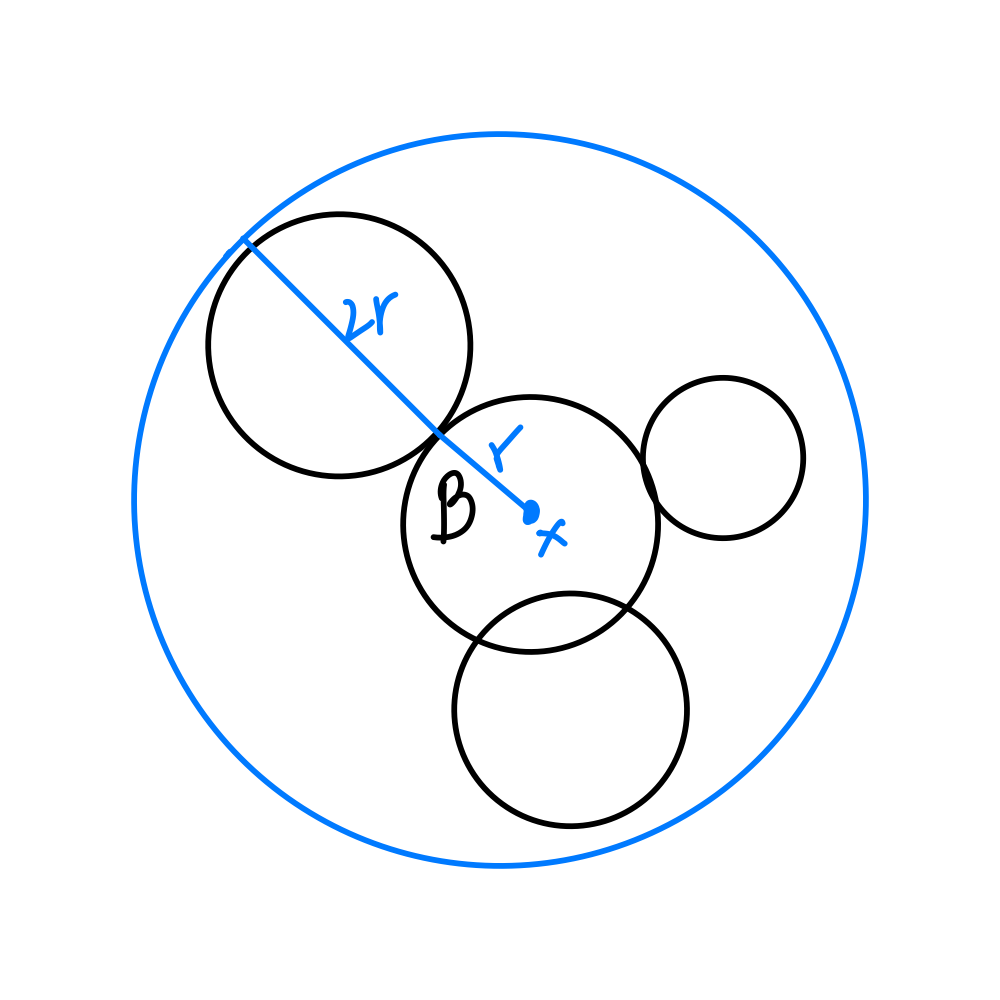
\includegraphics[width=0.4\linewidth,height=\textheight,keepaspectratio]{assets/main--figure-raster-022.png}

\end{center}

(每次都选择下一个和前面所有更大的球不 intersect 的最大球; 在这个过程中, 所有和前面更大的球有 intersection 的球都被被包括在该球的三倍球里.)

\end{proof}

\subsection{Hardy-Littlewood maximal theorem}\label{hardy-littlewood-maximal-theorem}

\begin{theorem}{\protect\phantomsection\label{kn-hl-maximal-theorem}{\textbf{HL maximal
theorem}}}

For \(L^{1}(m^{n})\), take constant \(C := 3^{n}\), 则对于任意 \(f \in L^{1}(m^{n})\), 都有:

\[\left. m(\left\{ {x:Hf(x) > \alpha} \right\}) \leq \frac{C}{\alpha}\int \middle| f| \right.\]

\end{theorem}

\begin{proof}

Set

\[E_{\alpha}: = \left\{ {x:Hf(x) > \alpha} \right\} \subset {\mathbb{R}}^{n}\]

因而 by def of \(Hf\), 对于任意的 \(x \in E_{\alpha}\) 都存在 \(r_{x}\) 使得

\[\left. m(B(x,r_{x})) < \frac{1}{\alpha}\int_{B(x,r_{x})} \middle| f| \right.\]

对于 compact \(K \in E_{\alpha}\), 一定存在 finite subcovering \(\left\{ {B(x_{i},r_{i})} \right\}\) covers \(K\).\\
于是 Apply Vitali-type covering Lemma:

\[\left. m(K) \leq \sum\limits_{i}m(3B(x_{i},r_{i})) = 3^{n}\sum\limits_{i}m(B(x_{i},r_{i})) \leq \frac{3^{n}}{\alpha}\int \middle| f| \right.\]

于是 by inner regularity, taking sup over all compact subsets 得证.

\end{proof}

\begin{qlremark}{Remark}

这是 HL max Thm 的一部分, 另一部分是 \(L^{p}\) space 下的. 这一部分表示了 HL maximal operator 的 \textbf{weakly boundedness}.\\
Notice: \(H\) 是一个从 \(L^{p}\) space (此处为 \(L^{1}\))到它自身的 (nonlinear) operator.\\
recall, 一个 operator 的 \textbf{(strongly) boundedness} 表示:

\[\left. | \middle| Tf \parallel \leq C \parallel f \parallel ,\quad\text{for all}\ f\ \text{(in the function space)} \right.\]

而 weakly boundedness 表示一定的可控制性: 越大的函数值, 能取到这个函数值的点的占比 (with respect to measure) 越小.\\
(will prove: \textbf{对于 \(p > 1\), \(H\) 具有 strongly boundedness}.)

\end{qlremark}

\begin{qlremark}{Remark}

我们可以 compare the HL ineq 和 Markov ineq. Markov ineq 表示, 对于任意 \(f \in L^{1}(\mu)\) 都有

\[\left. m(\left\{ {f > \alpha} \right\}) \leq \frac{1}{\alpha}\int \middle| f| \right.\]

\end{qlremark}

\section{Lebesgue differentiation Theorem {[}Fol 3.4{]}}

对应: Folland 3.4(2)

\begin{definition}{\protect\phantomsection\label{kn-lebesgue-set}{\textbf{Lebesgue set}}}

我们定义一个函数 \(f \in L_{loc}^{1}({\mathbb{R}}^{n})\) 的 Lebesgue set 为:

\[L_{f} := \left\{ x \in {\mathbb{R}}^{n} \mid \lim\limits_{r\rightarrow 0^{+}}\text{avg}_{B(x,r)} \middle| f(y) - f(x) \middle| dy = 0 \right\}\]

其中每个 point 被称为一个\textbf{Lebesgue point}.

\end{definition}

\begin{qlremark}{Remark}

一个 Lebesgue point \(x\) 即满足:

\[\left. \lim\limits_{r\rightarrow 0^{+}}A_{r} \middle| f - f(x) \middle| (x) = 0 \right.\]

同时可证明, 这个条件也等价于:

\[\lim\limits_{r\rightarrow 0^{+}}A_{r}f(x) = f(x)\]

即: \textbf{该点附近的 average value of \(f\) 等于 \(f\) 在改点的值.} 因为

\[\begin{matrix}
{A_{r}f(x) - f(x)} & {= \frac{1}{m(B(x,r))}\int_{B(x,r)}f dy - f(x)} \\
 & {= \frac{1}{m(B(x,r))}\int_{B(x,r)}f dy - \frac{f(x)}{m(B(x,r))}\int_{B(x,r)}1 dy} \\
 & {= \frac{1}{m(B(x,r))}\int_{B(x,r)}\lbrack f - f(x)\rbrack dy} \\
 & {= A_{r}\lbrack f - f(x)\rbrack(x)}
\end{matrix}\]

它是 \(\left. A_{r} \middle| f - f(x) \middle| (x) \right.\) 或其负数. 因而这两个函数趋向于 0 的趋势是相同的.

\end{qlremark}

\subsection{\texorpdfstring{original LDT: locally \(L^{1}\) 函数几乎每一点附近的函数均值都等于这一点上的值}{original LDT: locally L\^{}\{1\} 函数几乎每一点附近的函数均值都等于这一点上的值}}\label{original-ldt-locally-l1-ux51fdux6570ux51e0ux4e4eux6bcfux4e00ux70b9ux9644ux8fd1ux7684ux51fdux6570ux5747ux503cux90fdux7b49ux4e8eux8fd9ux4e00ux70b9ux4e0aux7684ux503c}

\begin{theorem}{\protect\phantomsection\label{kn-lebesgue-differentiation-theorem}{\textbf{Lebesgue
differentiation theorem}}}

对于任意的 \(f \in L_{loc}^{1}({\mathbb{R}}^{n})\), \(L_{f}\) is Leb mble and \(m(L_{f}^{c}) = 0\).

\end{theorem}

\begin{proof}

由于对于任意 \(x\) 都有:

\[f(x) = \lim\limits_{N\rightarrow\infty}f\chi_{B(0,N)}(x)\]

所以 it suffices to prove the statement for \(f\chi_{B(0,N)}\) for 任意 \(N\).\\
注意, \(f\chi_{B(0,N)}\) 是一个 \(L^{1}\) function. 因而只需要 prove the statement for \(f \in L^{1}({\mathbb{R}}^{n})\) 就可以 generalize it to \(f \in L_{loc}^{1}({\mathbb{R}}^{n})\). 因而 \textbf{WLOG suppose \(f \in L^{1}({\mathbb{R}}^{n})\)}.\\
首先, it is true for \(f \in C_{c}^{0}({\mathbb{R}}^{n})\). (容易 check: 在某点连续性的定义能够 imply 在这一点的均值等于这一点的值).\\
In other cases, 我们需要利用 \(C_{c}^{0}({\mathbb{R}}^{n})\) 在 \(L^{1}({\mathbb{R}}^{n})\) 中的 density.\\
Let

\[\left. Q(x,r): = A_{r} \middle| f - f(x) \middle| (x) \right.\]

这是一个 nonnegative function. 注意, 上个 lec 中我们证明了 \(A_{r}f(x)\) 是 jointly continuous in \(r\) and \(x\) 的. 因而 \(Q(x,r)\) 也是 jointly continuous in \(r\) and \(x\) 的.\\
我们随后定义:

\[Q(x): = \lim\sup\limits_{r\rightarrow 0^{+}}Q(x,r)\]

于是 \(x\mapsto Q\) 相当于 maximal function 的一个变体. 容易验证它也是 measurable 的. 我们 WTS:

\[m(\left\{ {x:Q(x) > 0} \right\}) = 0\]

等价于 show:

\[m(\left\{ {Q > \alpha} \right\}) = 0\quad\text{for all}\ \alpha = \frac{1}{n}, n \in {\mathbb{N}}\]

Let \(\epsilon > 0\). By density of \(C_{c}^{0}({\mathbb{R}}^{n})\) in \(L^{1}({\mathbb{R}}^{n})\), 我们可以 pick \(g \in C_{c}^{0}({\mathbb{R}}^{n})\) s.t.

\[\left. \int \middle| f - g \middle| < \epsilon \right.\]

By triangular ineq in \(L^{1}\), for a.e. \(x \in {\mathbb{R}}^{n}\) we have:

\[\left. A_{r} \middle| f - f(x) \middle| (x) \leq A_{r} \middle| f - g \middle| (x) + A_{r} \middle| g - g(x) \middle| (x) + A_{r} \middle| f(x) - g(x) \middle| (x) \right.\]

where

\[\left. \text{(constant)} A_{r} \middle| f(x) - g(x) \middle| (x) = \middle| f(x) - g(x)| \right.\]

因而 putting \(r\rightarrow 0^{+}\), we have \(\left. A_{r} \middle| f - f(x) \middle| (x)\rightarrow Q(x) \right.\), 以及 \(\left. A_{r} \middle| f - g \middle| (x)\rightarrow H(f - g)(x) \right.\); 从而上述不等式变为:

\[\left. Q(x) \leq H(f - g)(x) + 0 + \middle| f(x) - g(x)| \right.\]

从而一定有:

\[m(\left\{ {Q > \alpha} \right\}) \leq m(\left\{ {H(f - g) > \frac{\alpha}{2}} \right\}) + m(\left\{ |f - g \middle| > \frac{\alpha}{2} \right\})\]

我们分别以 HL max Thm 和 Chebyshev's Thm bound 住右边这两个式子, 得到:

\[\left. m(\left\{ {Q > \alpha} \right\}) \leq \frac{2 \cdot 3^{n}}{\alpha}\int \middle| f - g \middle| + \frac{2}{\alpha}\int \middle| f - g \middle| \leq \frac{2}{\alpha}(3^{n} + 1)\epsilon\overset{\epsilon\rightarrow 0}{\rightarrow}0 \right.\]

从而得证.

\end{proof}

\begin{corollary}

\[x \in L_{loc}^{1}({\mathbb{R}}^{n}))\Longrightarrow\lim\limits_{r\rightarrow 0^{+}}A_{r}f(x) = f(x) a.e.\]

\end{corollary}

\begin{proof}

If \(x \in L_{f}\) then

\[\left. |\ \text{avg}_{B(x,r)}(f(y) - f(x)) dy\  \middle| \leq \text{avg}_{B(x,r)} \middle| (f(y) - f(x) \middle| dy\overset{r\rightarrow 0}{\rightarrow}0 \right.\]

\end{proof}

\begin{qlremark}{Remark}

我们先前已经 verify 了: Lebesgue point 的定义 \(\left. \lim_{r\rightarrow 0^{+}}A_{r} \middle| f - f(x) \middle| (x) = 0 \right.\) 和 \(\lim_{r\rightarrow 0^{+}}A_{r}f(x) = f(x)\) 是等价的.\\
因而 Lebesgue Differentiation Thm 即表示: \textbf{locally \(L^{1}\) 函数几乎每一点附近的函数均值都等于这一点上的值.}\\
实则, locally \(L^{1}\) 是一个很宽松的条件. 基本上, 只要是 measurable function 且不要有过多的 unbounded points, 这个函数就是 locally \(L^{1}\) 的. 所以 \textbf{LDT 表示的是大多数可测函数几乎每一点附近的函数均值都等于这一点上的值.}\\

\end{qlremark}

\begin{qlremark}{Remark}

在 Hw 8 中将 prove LDT 的 \(L^{p}\) 版本: 对于任意 \(1 \leq p < \infty\), 如果 \(f \in L^{p}({\mathbb{R}})\), 都有

\[\left. \lim\limits_{r\rightarrow 0}\frac{1}{2r}\int_{x - r}^{x + r} \middle| f(y) - f(x) \middle| {}_{p} dy = 0\quad\text{for}\ a.e.x \right.\]

\end{qlremark}

\subsection{density of a set at a point}\label{density-of-a-set-at-a-point}

\begin{definition}{\protect\phantomsection\label{kn-density-of-a-set-at-a-point}{\textbf{density
of a set at a point}}}

对于 \(E \subset {\mathbb{R}}^{n}\) Lebesgue measurable (which implies: \(\chi_{E} \in L_{loc}^{1}\)), 我们定义:

\[D_{E}(x): = \lim\limits_{r\rightarrow 0^{+}}\frac{m(E \cap B(x,r))}{m(B(x,r))}\]

\end{definition}

\begin{qlremark}{Remark}

density, 一个点附近一个集合占的密度, 理解很直观.\\

\begin{center}

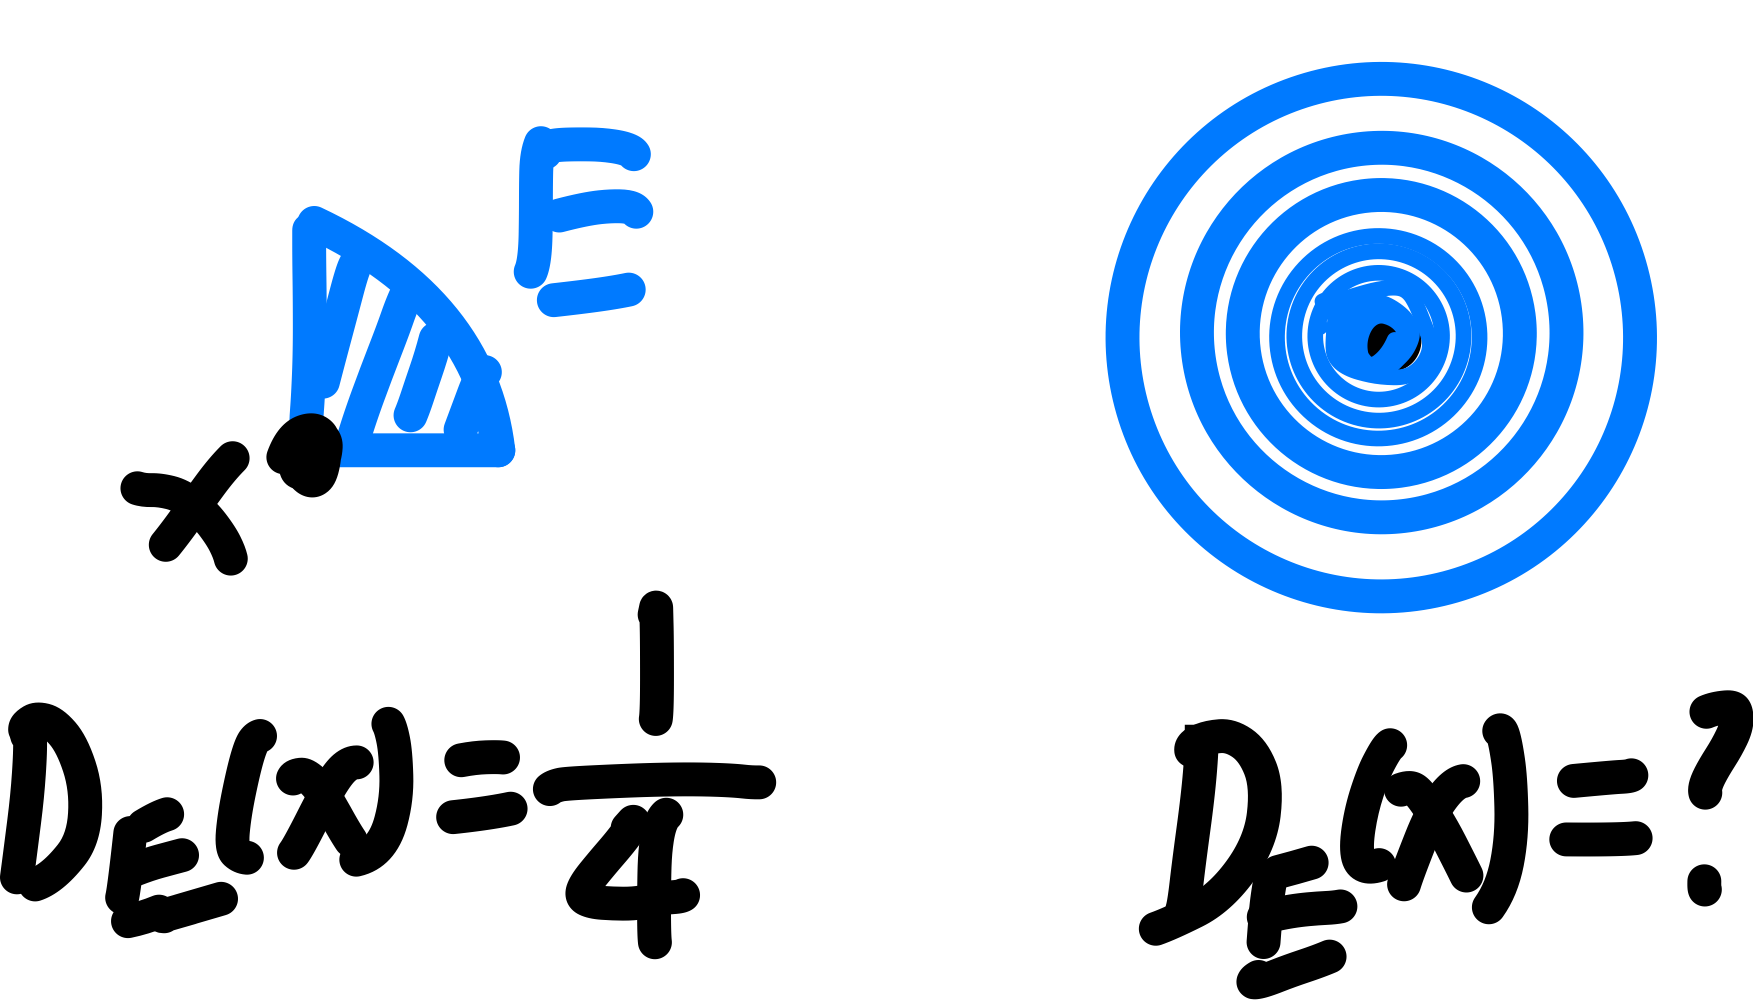
\includegraphics[width=0.3\linewidth,height=\textheight,keepaspectratio]{assets/main--figure-raster-023.png}

\end{center}

这是一个极限行为, 表示这个集合在这个点附近 locally 占的比例趋向于的极限.\\
如果是一个分布连续的集合, 比如一个扇形等, 那么就很好求. 但是如果是右图这样分布比较断断续续的集合, 会需要仔细考虑极限.\\
不过, LDT 告诉我们:

\end{qlremark}

\begin{corollary}

对于\(E \subset {\mathbb{R}}^{n}\) Lebesgue measurable (which implies: \(\chi_{E} \in L_{loc}^{1}\)), 一定有:

\[\begin{matrix}
{D_{E}(x) = \{ 1,\quad\text{for a.e.}\ x \in E} \\
{0,\quad\text{for a.e.}\ x \in E^{c}}
\end{matrix}\]

\end{corollary}

\begin{proof}

因为这个 indicator function 是 measurable 的, 以及 locally \(L^{1}\) 的. 所以\textbf{它在 \(x\) 处的 density 就变成了它在 \(x\) 处的均值}, 从而在 \(E\) 上 a.e. 为 1, 在 \(E^{c}\) 上 a.e. 为 0 (函数值).

\end{proof}

\begin{example}

我们这里介绍一些 behavior 比较特殊的集合, 空间每点上这个集合的 density.\\
考虑

\[E: = \left\{ 0 \right\} \cup \bigcup\limits_{j = 0}^{\infty}\lbrack\frac{2}{3} \cdot \frac{1}{2^{j}},\frac{1}{2^{j}}\rbrack\]

这是一个 closed set.\\

\begin{center}

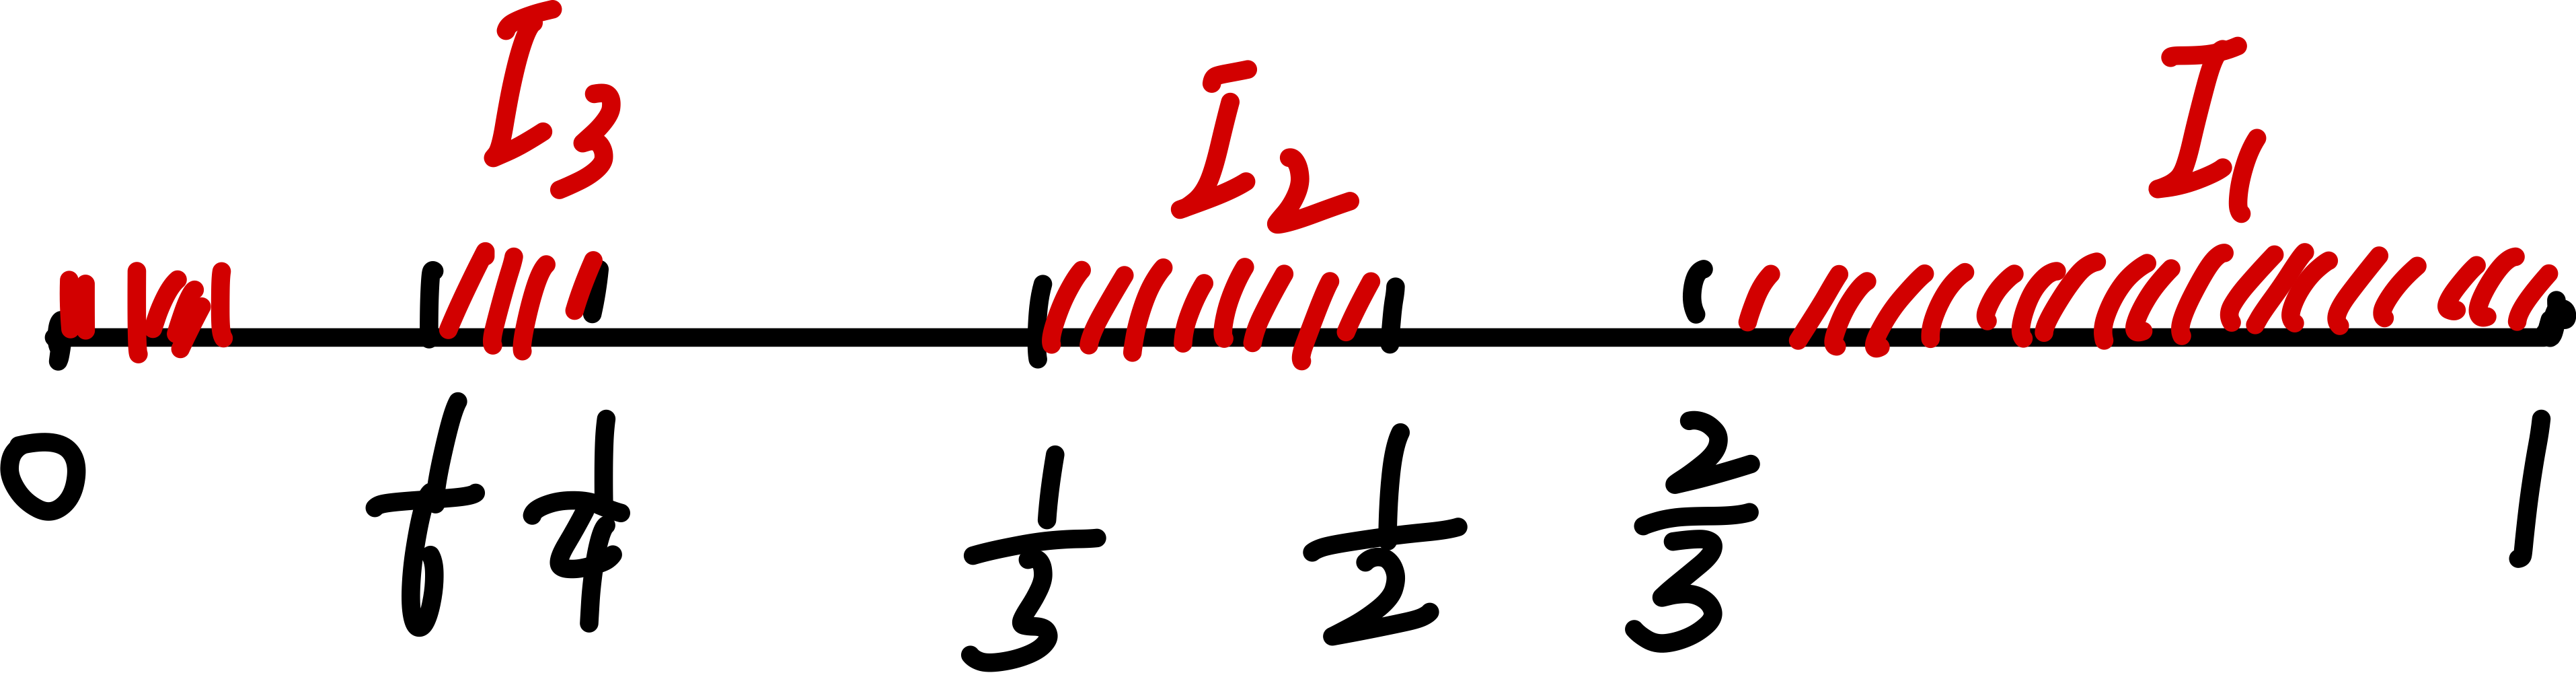
\includegraphics[width=0.4\linewidth,height=\textheight,keepaspectratio]{assets/main--figure-raster-024.png}

\end{center}

对于 \(x \in E^{\circ}\), \(D_{E}(x) = 1\).\\
对于 \(x \notin E\), \(D_{E}(x) = 0\).\\
对于 \(x \in \partial E\), \(D_{E}(x) = \frac{1}{2}\). (区间的一边在 \(E\) 里, 一边不在 \(E\) 里)\\
对于 \(x \in 0\), \(D_{E}(0)\) \textbf{undefined}. 因为每段空心和实心的地方, 这个比例的落差都非常大. (容易证明这个极限不存在.)\\
而反观, 任取 \(\alpha \in (0,1)\), 那么取

\[E := \bigcup\limits_{n = 1}^{\infty}(\frac{1}{n},\frac{1}{n} + \frac{\alpha}{n(n - 1)})\]

则有:

\[D_{E}(0) = \frac{\alpha}{2}\]

\begin{center}

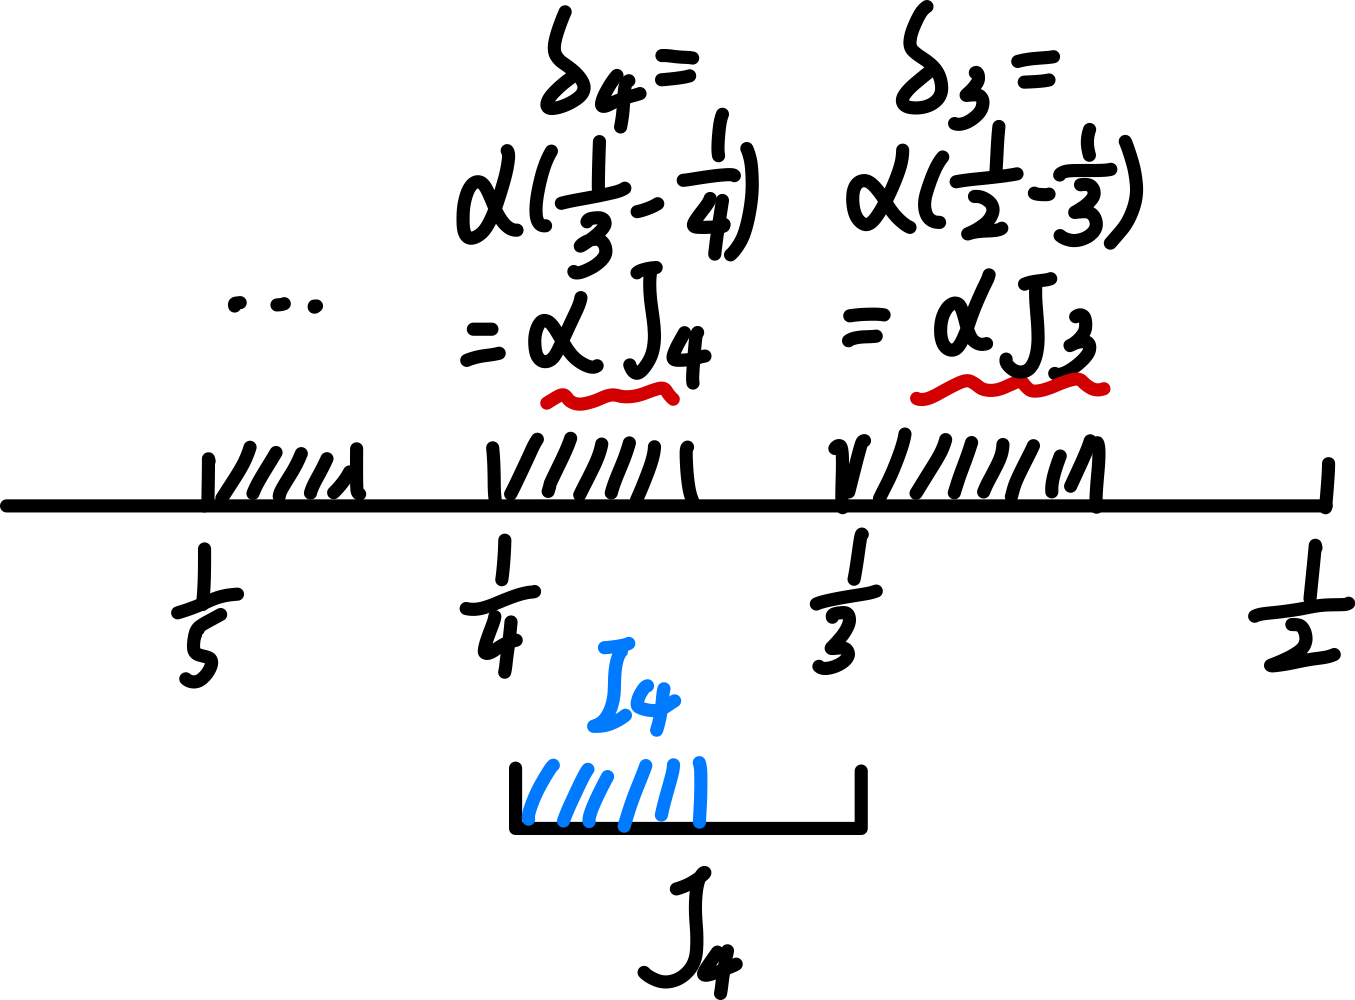
\includegraphics[width=0.4\linewidth,height=\textheight,keepaspectratio]{assets/main--figure-raster-025.png}

\end{center}

这里的关键在于，harmonic seq 随着 \(n\) 的增长而缩小的速度非常慢. 在 \(n\) 较大的情况下, 背景区间 \(J_{n}\) 几乎与 \(J_{n + 1}\) 具有相同的长度, 因此正如我们所知，\(m(J_{n})/m( \cup_{k > N}J_{k}) = 0\). 所以, 无论 \(r\) 位于实心部分 \(I_{n}\) 还是空心部分 \(J_{n}\backslash I_{n}\) 都不太重要.\\
另一方面, 我们刚才的例子使用 geometric seq 作为背景区间 \(J_{n}\) 的构建块, 则 fail, 因为 \(J_{n}\) 的长度与 \(\cup_{k \geq n}J_{k}\) 相比太大了, 有 \(m(J_{n}) = m( \cup_{k > n}J_{k})\), 因此无论 \(r\) 位于实心区间还是空心区间 这使得 \(0\) 处的密度无法定义.

\end{example}

\subsection{generalized LDT}\label{generalized-ldt}

genralized LDT 表示\textbf{对形状不规则 (未必是 ball) 的收敛行为}, LDT 的 statement 仍然 stay true. 即, \textbf{只要 a family of Lebesgue mble sets \(E_{r}\) shrink nicely to \(x\), LDT 就满足.}

\begin{theorem}{\protect\phantomsection\label{kn-generalized-ldt}{\textbf{generalized
LDT}}}

对于 \(f \in L_{loc}^{1}({\mathbb{R}}^{n})\), 任意的 \(x \in L_{f}\), 令 \(\left\{ {E_{r}(x)} \right\}\) 为 a family of Lebesgue measurable sets, 其中对于每个 \(E_{r}(x)\) 都有:

\[E_{r}(x) \subset B(x,r)\]

并且

\[m(E_{r}(x)) > \alpha m(B(x,r))\]

for some \(0 < \alpha < 1\).\\
则有:

\[\lim\limits_{r\rightarrow 0^{+}}\frac{\left. \int_{E_{r}(x)} \middle| f(y) - f(x) \middle| dy \right.}{m(E_{r}(x)} = 0\quad\text{for a.e.}\ x\]

\end{theorem}

证明很简单, 因为

\[\lim\limits_{r\rightarrow 0^{+}}\frac{\left. \int_{E_{r}(x)} \middle| f(y) - f(x) \middle| dy \right.}{m(E_{r}(x))} \leq \lim\limits_{r\rightarrow 0^{+}}\frac{\left. \int_{B(x,r)} \middle| f(y) - f(x) \middle| dy \right.}{m(E_{r}(x))} \leq \lim\limits_{r\rightarrow 0^{+}}\frac{\left. \int_{B(x,r)} \middle| f(y) - f(x) \middle| dy \right.}{\alpha m(B(x,r))} = 0\]

\begin{qlremark}{Remark}

LDT 最重要的作用是之一定义了在 \textbf{Lebesgue 积分理论下的一种形式的 FTC:}

\begin{theorem}{\protect\phantomsection\label{kn-ftc-in-lebesgue}{\textbf{FTC in
Lebesgue}}}

对于 \(f \in L_{loc}^{1}({\mathbb{R}})\), 任取 \(x \in L_{f}\), 都有

\[\lim\limits_{r\rightarrow 0}\frac{1}{r}\int_{x}^{x + r}f dm = f(x)\]

\end{theorem}

更 generally, 它表示由一个函数 \(f\) 在 measurable set 上对 measure \(m\) 的积分值定义出来的 measure \(\nu\) ,对于 \(m\) 的 Radon-Nikodym 导数.

\[\lim\limits_{r\rightarrow 0^{+}}\frac{\nu(E_{r})}{m(E_{r})} = f(x)\]

表示了 Euclidean space 上, 从 measure 比的极限恢复 Radon-Nikodym 导数的方法.\\
之后系统学习 Radon-Nikodym Theory, 将详细展开, 并引入更多的不等式和 FTC 形式. 而我们接下来将先展开 \(L^{p}\) space theory.

\end{qlremark}
\end{document}
